\documentclass[10pt,a4paper]{article}
\usepackage[top=19mm,bottom=25.4mm,left=16mm,right=16mm]{geometry}
\usepackage{fontspec,graphicx,amsmath,amssymb,multicol,booktabs,array,tabularx}
\usepackage[hidelinks]{hyperref}
\setmainfont{Times New Roman}
\setlength{\columnsep}{6mm}
\setlength{\parindent}{0pt}
\setlength{\parskip}{3pt}
\setlength{\multicolsep}{4pt}
\setlength{\abovedisplayskip}{4pt}
\setlength{\belowdisplayskip}{4pt}
\pagestyle{empty}
\makeatletter
\renewcommand{\section}{\@startsection{section}{1}{0pt}{5pt}{2pt}{\normalfont\normalsize\bfseries}}
\makeatother
\newcommand{\sect}[1]{\section*{#1}}
\begin{document}
\begin{center}
\includegraphics[width=\textwidth]{baic2026_header.png}\par\vspace{4pt}
{\fontsize{14}{17}\selectfont\bfseries Hard-Budget Feature Selection with Resampled Mutual-Information Repair in EHOA}\par
Amirreza Ghaffarian\par
Graduate Student, Islamic Azad University\end{center}
\textbf{Abstract. } Fold-local budget repairs in EHOA were evaluated in 750 primary and 714 sensitivity runs. Resampled repair gives balanced accuracy (BA) 0.7932, synthetic cost ratio 0.2774 and descriptive stability 0.2241 across ten datasets. Another 450 post-hoc no-search fits give BA/stability 0.7869/0.6709 for MI deletion and 0.7840/0.7999 for resampled deletion. Neither BA contrast is Holm-significant. Stability significance versus original EHOA disappears in every nine-dataset omission analysis. EHOA necessity is unestablished. Separate three-feature transfer gives subject-level BA 0.575 [descriptive 95\% interval 0.475,0.675] on 80 subjects. Synthetic costs and shared FNA fees do not establish clinical savings or validate the original 22-feature model.

\textbf{Keywords. } feature selection, hard budget, resampled mutual information, subset stability
\begin{multicols}{2}\raggedcolumns
\sect{1  Problem and contribution}
Small subsets need not be inexpensive. Hard budgets limit selected acquisition costs [1]; subset stability measures variation in selected identities, separately from accuracy or convergence [2].

Medical feature selection [3] separates predictive discrimination, reproducible feature identity and acquisition burden. Correlated descriptors may substitute for each other; repeated selection does not validate a biomarker.

We retain EHOA search [4] and change repair utility only. The contribution is an auditable controlled comparison, not a new optimization family or established clinical tool.

\sect{2  Related studies}
Stability need not imply useful predictors [5]. Penalized medical selection [6], sequential acquisition [7] and grouped costs [8] address different settings (Table 1); their numerical results are not directly comparable. NR means not reported in the inspected source.

\par\vspace{3pt}\begin{minipage}{\linewidth}{\footnotesize Table 1. Related-work comparison. Full evaluation details are in the supplement.\par}
{\fontsize{6.8}{8.3}\selectfont\setlength{\tabcolsep}{2pt}\renewcommand{\arraystretch}{1.1}
\begin{tabularx}{\linewidth}{>{\hsize=1.0000\hsize\raggedright\arraybackslash}X>{\hsize=1.0000\hsize\raggedright\arraybackslash}X>{\hsize=1.0000\hsize\raggedright\arraybackslash}X>{\hsize=1.0000\hsize\raggedright\arraybackslash}X>{\hsize=1.0000\hsize\raggedright\arraybackslash}X>{\hsize=1.0000\hsize\raggedright\arraybackslash}X}\toprule
Study & Budget & Costs & Stability & Evaluation & Difference\\\midrule
Jagdhuber [1] & Yes & Additive & NR & Simulation & Feasible GA\\
Nogueira [2] & NR & NR & Chance-corrected & Resampling & Metric\\
Hamer [5] & NR & NR & Importance-weighted & Resampling & Metric limits\\
Klonecki [6] & Yes & Feature / proxy & NR & Medical data & Penalized ERM\\
Valancius [7] & NR & Sequential & NR & AFA benchmarks & Patient-wise policy\\
Klonecki [8] & Yes & Grouped & NR & MIMIC & Shadow stopping\\
This work & Yes & Synthetic additive & Nogueira & 5 x 3 outer & MI/cost repair\\
\bottomrule\end{tabularx}}
\end{minipage}\par\vspace{3pt}
Classical stability selection aggregates repeated subsample selections and, under specified assumptions and thresholds, controls false selections [9,10]. Our four MI resamples instead estimate a deletion utility before wrapper search. We neither threshold repeated selection probabilities nor inherit those error-control guarantees. Nogueira stability evaluates the final masks [2]; it is not the optimized fitness. Active acquisition [7] chooses measurements sequentially per case, whereas our repair returns a fixed feasible subset.

\sect{3  Implemented EHOA}
Each hiker has a continuous position x and a velocity v; a binary mask z selects features. Initialization uses a tent sequence with initial value 0.7 and parameter 0.4, mapped to [-6,6]. Velocities start uniformly in [-1.2,1.2]. For iteration t of T=10, the implemented update is:

\begin{equation}\begin{gathered}\begin{aligned}v_i\leftarrow\operatorname{clip}_{[-12,12]}\big(&w_t v_i+SF_t[2r_1(p_i-x_i)\\&+2r_2(g-x_i)]\big)\end{aligned}\end{gathered}\end{equation}
\begin{equation}\begin{gathered}\begin{gathered}x_i\leftarrow\operatorname{clip}_{[-6,6]}(x_i+v_i)\\w_t=0.9-0.5t/T,\quad SF_t=3-2t/T\end{gathered}\end{gathered}\end{equation}
Here p\_i and g are personal and global best continuous positions, and r\_1,r\_2 are independent per-feature uniform draws. The sigmoid gives selection probability 1/(1+exp(-x\_j)); an empty sampled mask restores the largest probability. The implementation keeps continuous leaders separate from repaired masks, caches fitness for duplicate masks, and stops after ten iterations without early stopping.

\sect{4  Fold-local budget repair and stability}
Costs are fixed positive synthetic additive units, drawn with NumPy seed 1000+D from lognormal(0,0.7). The primary budget is B=0.30 sum(c); sensitivity uses 0.15 and 0.50. Costs are independent of labels and do not represent money. Every constrained nonempty mask must satisfy sum(z\_j c\_j)<=B. Shared acquisition costs require a different grouped model [6,8]. There is only one cost assignment per dimension; equal-dimensional datasets share that vector. Results are conditional on this assignment. Utility/cost ratios can favor cheap noise [18].

\begin{equation}\begin{gathered}u_j=\max(0,\overline I_j-\lambda s_j),\quad q_j=u_j/c_j\end{gathered}\end{equation}
For each inner fold, MI is fitted to its imputed training rows only. Four class-stratified samples draw ceil(0.8 n\_class) rows with replacement (minimum two). The continuous-discrete estimator uses three neighbors [11]; Dermatology treats its first 33 categorical/ordinal inputs as discrete and age as continuous. MI is in nats and s\_j is sample SD. Lambda=1 gives a conservative utility, not a calibrated confidence bound; there is no division by sqrt(R). Final outer-training utility is separate and never used to repair inner-validation candidates. Parkinson utility resamples recordings, not subjects; SD is not subject-level uncertainty.

\par\vspace{3pt}\begin{minipage}{\linewidth}{\footnotesize Table 2. Four repairs share the same deletion rule.\par}
{\fontsize{6.8}{8.3}\selectfont\setlength{\tabcolsep}{2pt}\renewcommand{\arraystretch}{1.1}
\begin{tabularx}{\linewidth}{>{\hsize=1.0000\hsize\raggedright\arraybackslash}X>{\hsize=1.0000\hsize\raggedright\arraybackslash}X>{\hsize=1.0000\hsize\raggedright\arraybackslash}X}\toprule
Repair & Utility u\_j & Meaning\\\midrule
Random/cost & U(0,1), fixed per training fold & Not uniform deletion\\
Cheapest & 1 & Largest cost first\\
MI/cost & Single-sample MI & Relevance per cost\\
Resampled/cost & max(0, mean MI - SD) & Conservative heuristic\\
\bottomrule\end{tabularx}}
\end{minipage}\par\vspace{3pt}
Search samples a raw mask. Each inner fold repairs this candidate with its own training utility, then fits imputation, scaling and SMOTE on the selected columns [12]. Validation rows are only transformed and predicted. Fitness averages ordinary accuracy and selected size across three independently repaired folds. The winning raw candidate is finally repaired with outer-training utility; inner and final masks may differ. The outer classifier is refitted using only final selected columns. This evaluates a complete selection-and-repair procedure, not a fixed mask reused across all inner folds [13].

\begin{equation}\begin{gathered}\begin{gathered}F(z)=\frac13\sum_{f=1}^3F_f(z)\\F_f(z)=0.99(1-Acc_f)+0.01k_f/D\end{gathered}\end{gathered}\end{equation}
Deletion removes the active feature minimizing utility/cost while over budget. An unaffordable singleton is cleared; an empty mask restores the affordable highest-ratio feature. Positive costs and finite deletion ensure feasibility when one feature is affordable, as verified here. This guarantees budget compliance, not optimal prediction. MI remains marginal and can overlook interactions or redundancy.

\begin{equation}\begin{gathered}\Phi=\operatorname{clip}_{[-1,1]}\left(1-\frac{\frac M{M-1}\frac1D\sum_j p_j(1-p_j)}{(\bar k/D)(1-\bar k/D)}\right)\end{gathered}\end{equation}
Nogueira stability [2] uses M=15 final masks per dataset/configuration, selection frequencies p\_j and mean size k-bar. Identical full/empty masks return one in the code. The masks overlap in training data and are dependent; their copied stability values are not fifteen independent observations. Jaccard is a supplementary, uncorrected overlap measure.

\sect{5  Datasets and source corrections}
\par\vspace{3pt}\begin{minipage}{\linewidth}{\footnotesize Table 3. Fresh-run dataset specifications; U links to archive.ics.uci.edu/dataset/\{id\}.\par}
{\fontsize{6.8}{8.3}\selectfont\setlength{\tabcolsep}{2pt}\renewcommand{\arraystretch}{1.1}
\begin{tabularx}{\linewidth}{>{\hsize=1.8947\hsize\raggedright\arraybackslash}X>{\hsize=0.5684\hsize\raggedright\arraybackslash}X>{\hsize=0.3789\hsize\raggedright\arraybackslash}X>{\hsize=0.3789\hsize\raggedright\arraybackslash}X>{\hsize=2.1474\hsize\raggedright\arraybackslash}X>{\hsize=0.6316\hsize\raggedright\arraybackslash}X}\toprule
Dataset & N & D & K & Class counts & Source\\\midrule
Breast Cancer & 569 & 30 & 2 & 212/ 357 & U17\\
Wine & 178 & 13 & 3 & 59/ 71/ 48 & U109\\
Ionosphere & 350 & 34 & 2 & 125/ 225 & U52\\
Sonar & 208 & 60 & 2 & 111/ 97 & U151\\
Dermatology & 366 & 34 & 6 & 112/ 61/ 72/ 49/ 52/ 20 & U33\\
Spambase & 4210 & 57 & 2 & 2531/ 1679 & U94\\
Parkinson (grouped) & 195 & 22 & 2 & 48/ 147 & U174\\
Hill Valley & 1212 & 100 & 2 & 606/ 606 & U166\\
Steel (corrected) & 1941 & 27 & 7 & 158/ 190/ 391/ 72/ 55/ 402/ 673 & U198\\
Madelon & 2600 & 500 & 2 & 1300/ 1300 & U171\\
\bottomrule\end{tabularx}}
\end{minipage}\par\vspace{3pt}
Exact (X,y) duplicates are removed: Ionosphere uses 350 rows and Spambase 4210. Steel removes six target-indicator inputs and reconstructs seven fault classes. Parkinson recordings match the UCI numeric file and use 32 subject prefixes in both outer and inner group splits. The UCI narrative states 31 participants, so clinical group identity remains unverified. Original raw data and earlier results are preserved. Six Spambase rows form three identical-feature, opposite-label pairs; 94/114 runs split a pair across outer folds. Email identities are unknown; feature collision does not establish entity leakage.

\sect{6  Fresh protocol and statistical analysis}
The first fold-safe study used three seeds; two additional seeds give five (72001-72005), three outer folds and 750 primary runs across ten datasets and five methods. The extension protocol and code hashes were published in GitHub commit 72c87b6 before its 690 runs: 300 seed replications, 240 complete factorial runs and 150 larger-search runs. Earlier outcomes were known. This is prospective versioning, not an independent formal preregistration or registration of past experiments. Inner utility uses training labels only; outer tests are never used to choose a parameter winner.

\par\vspace{3pt}\begin{minipage}{\linewidth}{\footnotesize Table 4. Actual frozen settings.\par}
{\fontsize{6.8}{8.3}\selectfont\setlength{\tabcolsep}{2pt}\renewcommand{\arraystretch}{1.1}
\begin{tabularx}{\linewidth}{>{\hsize=1.0000\hsize\raggedright\arraybackslash}X>{\hsize=1.0000\hsize\raggedright\arraybackslash}X}\toprule
Parameter & Value\\\midrule
Population / iterations & Primary 8/10; search study 16/20\\
Position / velocity clip & [-6,6] / [-12,12]\\
Tent / sweep / inertia & 0.7,p=0.4 / 3 to 1 / 0.9 to 0.4\\
c1,c2 / alpha & 2,2 / 0.99\\
Outer / inner folds & 3 / 3; Parkinson grouped\\
Outer seeds & 72001-72005\\
Selector seed & outer seed + fold index x 100003\\
Primary R / fraction / lambda & 4 / 0.8 with replacement / 1\\
Sensitivity R / lambda & Factorial 4,8 / 0,2; earlier OFAT 4,8,16 / 0,1,2\\
Cost / budgets & lognormal(0,0.7) / 15,30,50\%\\
Classifier & 5-NN; uniform; Euclidean\\
Imputation / scale / SMOTE & Training-selected columns only\\
Timing & Includes utility and final classification\\
\bottomrule\end{tabularx}}
\end{minipage}\par\vspace{3pt}
Each dataset is one statistical block [14]. Ten-block Friedman uses df=4; two-sided Wilcoxon contrasts have within-metric and Holm24 corrections, plus six corrected omnibus tests. Seed-20261012 dataset bootstrap uses 20000 draws; intervals are descriptive and unadjusted. Fifteen dependent masks are not independent replicates.

\sect{7  Results and sensitivity}
\par\vspace{3pt}\begin{minipage}{\linewidth}{\footnotesize Table 5. Equal-weight dataset means. First five rows: original primary study; last three: post-hoc no-search controls. V is budget exceedance; full-mask stability 1 is a degenerate convention.\par}
{\fontsize{6.8}{8.3}\selectfont\setlength{\tabcolsep}{2pt}\renewcommand{\arraystretch}{1.1}
\begin{tabularx}{\linewidth}{>{\hsize=1.0000\hsize\raggedright\arraybackslash}X>{\hsize=1.0000\hsize\raggedright\arraybackslash}X>{\hsize=1.0000\hsize\raggedright\arraybackslash}X>{\hsize=1.0000\hsize\raggedright\arraybackslash}X>{\hsize=1.0000\hsize\raggedright\arraybackslash}X>{\hsize=1.0000\hsize\raggedright\arraybackslash}X}\toprule
Method & BA & Cost ratio & Size & Stability & V\\\midrule
EHOA & 0.7946 & 0.4947 & 42.84 & 0.1036 & 145/150\\
Random/cost & 0.7814 & 0.2724 & 31.59 & 0.1217 & 0/150\\
Cheapest & 0.7944 & 0.2765 & 35.05 & 0.2476 & 0/150\\
MI/cost & 0.7949 & 0.2787 & 27.31 & 0.2203 & 0/150\\
Resamp./cost & 0.7932 & 0.2774 & 31.24 & 0.2241 & 0/150\\
Greedy MI & 0.7869 & 0.2772 & 34.23 & 0.6709 & 0/150\\
Greedy resamp. & 0.7840 & 0.2829 & 41.18 & 0.7999 & 0/150\\
All features & 0.7873 & 1.0000 & 87.70 & 1.0000 & 150/150\\
\bottomrule\end{tabularx}}
\end{minipage}\par\vspace{3pt}
Post-hoc controls add 450 fits on identical outer splits. Each filter repairs an all-ones mask once using saved training-only utility, without search or test tuning. Resampled EHOA minus MI/resampled/all-feature controls has BA deltas +0.00630/+0.00926/+0.00594 (Holm9 p=0.7734/0.9668/1). Stability deltas versus filters are -0.44678/-0.57580 (Holm9 p=0.02344/0.01758). A conservative post-result Holm33 sensitivity combining original and new contrasts gives p=0.08203/0.06445 for these stability contrasts; none of the new contrasts survives. All-feature cost/stability are mechanical. Supplementary dataset means and unadjusted intervals avoid equivalence or standalone-runtime claims.

\par\vspace{3pt}\begin{minipage}{\linewidth}{\footnotesize Table 6. Friedman and mean ranks in E/R/C/M/S order; lower rank is better.\par}
{\fontsize{6.8}{8.3}\selectfont\setlength{\tabcolsep}{2pt}\renewcommand{\arraystretch}{1.1}
\begin{tabularx}{\linewidth}{>{\hsize=1.0000\hsize\raggedright\arraybackslash}X>{\hsize=1.0000\hsize\raggedright\arraybackslash}X>{\hsize=1.0000\hsize\raggedright\arraybackslash}X>{\hsize=1.0000\hsize\raggedright\arraybackslash}X>{\hsize=1.0000\hsize\raggedright\arraybackslash}X>{\hsize=1.0000\hsize\raggedright\arraybackslash}X>{\hsize=1.0000\hsize\raggedright\arraybackslash}X>{\hsize=1.0000\hsize\raggedright\arraybackslash}X}\toprule
Metric & Chi2 & p & E & R & C & M & S\\\midrule
BA & 6.8800 & 0.14237 & 2.50 & 4.10 & 2.60 & 2.70 & 3.10\\
Cost & 21.2000 & 0.00029 & 5.00 & 2.20 & 2.60 & 2.90 & 2.30\\
Size & 29.1313 & <0.00001 & 5.00 & 1.85 & 3.55 & 1.75 & 2.85\\
Stability & 29.6800 & <0.00001 & 4.70 & 4.20 & 1.60 & 2.20 & 2.30\\
\bottomrule\end{tabularx}}
\end{minipage}\par\vspace{3pt}
Resampled minus EHOA gives BA delta -0.00141 (W=22, within-metric Holm p=1, r=-0.200; descriptive 95\% interval [-0.01024,0.00799]). Stability delta is +0.12045 (Holm24 p=0.04688); predictive superiority is unestablished.

All ten post-hoc nine-dataset omission analyses retain positive stability deltas but lose Holm24 significance (Table 7). The minimum two-sided signed-rank p is 2/512, so minimum Holm24 is 0.09375. This is threshold fragility, not proof of no effect; no omitted dataset selects a winner.

\par\vspace{3pt}\begin{minipage}{\linewidth}{\footnotesize Table 7. Post-hoc stability robustness, Resampled minus EHOA; intervals across omissions are ranges, not confidence intervals.\par}
{\fontsize{6.8}{8.3}\selectfont\setlength{\tabcolsep}{2pt}\renewcommand{\arraystretch}{1.1}
\begin{tabularx}{\linewidth}{>{\hsize=1.1594\hsize\raggedright\arraybackslash}X>{\hsize=0.2899\hsize\raggedright\arraybackslash}X>{\hsize=1.6232\hsize\raggedright\arraybackslash}X>{\hsize=0.9275\hsize\raggedright\arraybackslash}X}\toprule
Analysis & N & Stability delta & Holm24 p\\\midrule
Original & 10 & +0.12045 & 0.04688\\
No Oxford & 9 & +0.12035 & 0.09375\\
Each omission & 9 & [+0.10487,+0.12842] & >=0.09375\\
\bottomrule\end{tabularx}}
\end{minipage}\par\vspace{3pt}
The complete 2x2x2 factorial crosses budget 0.15/0.50, R=4/8 and lambda=0/2 on all ten datasets. Orthogonal contrasts estimate main, pairwise and three-way endpoint effects. Each cell has one seed and three outer folds, so interactions are descriptive and do not cover the full continuous parameter space. A paired larger-search study compares 16 hikers and 20 iterations with 8 and 10 using seed 72001, shared outer splits and all five methods. All configurations were reported; none was selected from outer-test results.

Cheapest repair is more stable than resampled EHOA (0.2476 versus 0.2241); no corrected advantage over MI or cheapest is established. The primary contrast changes both MI averaging and SD penalization, so it does not isolate the SD contribution at 30\% budget.

The endpoint R=8 versus R=4 balanced-accuracy effect is +0.00786, averaged over budgets and penalties, with descriptive interval [0.00154,0.01527]. Larger search changes resampled inner fitness by -0.01554, but its outer BA delta is -0.00424, interval [-0.02869,0.01940]. Thus better optimized inner fitness does not establish better held-out prediction. These intervals are unadjusted descriptive contrasts; they do not select the primary setting.

\par\begin{minipage}{\linewidth}\centering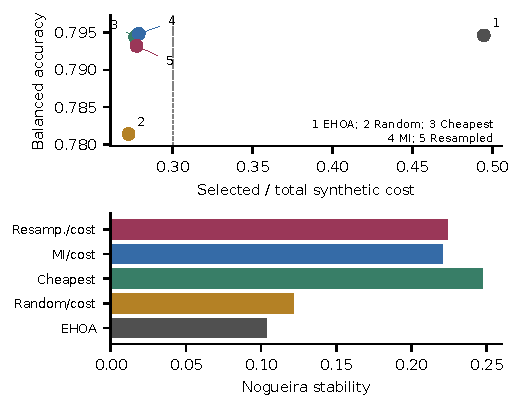
\includegraphics[width=\linewidth]{figures/eligible_comparison.pdf}\par{\footnotesize Figure 1. Fresh ten-dataset means; synthetic cost and descriptive subset stability.\par}\end{minipage}\par
\sect{8  Biomedical case and congress relevance}
Breast Cancer Wisconsin (Diagnostic) has 569 fine-needle-aspirate cases, 212 malignant and 357 benign, with 30 nuclear-image descriptors [15]. Table 8 and Figure 2 show fifteen masks per method. Counts describe computational selections, not causal biomarkers. Several descriptors share the same image acquisition, so additive synthetic costs cannot be interpreted as biopsy-price savings. Label 0 is malignant and label 1 benign; class-specific recall is explicitly reported.

\par\vspace{3pt}\begin{minipage}{\linewidth}{\footnotesize Table 8. Breast-cancer case: fifteen runs per method.\par}
{\fontsize{6.8}{8.3}\selectfont\setlength{\tabcolsep}{2pt}\renewcommand{\arraystretch}{1.1}
\begin{tabularx}{\linewidth}{>{\hsize=1.0000\hsize\raggedright\arraybackslash}X>{\hsize=1.0000\hsize\raggedright\arraybackslash}X>{\hsize=1.0000\hsize\raggedright\arraybackslash}X>{\hsize=1.0000\hsize\raggedright\arraybackslash}X>{\hsize=1.0000\hsize\raggedright\arraybackslash}X>{\hsize=1.0000\hsize\raggedright\arraybackslash}X}\toprule
Method & BA & Mal. sens. & Ben. spec. & Cost & Stability\\\midrule
EHOA & 0.9512 & 0.9415 & 0.9608 & 0.5620 & 0.0727\\
Random/cost & 0.9382 & 0.9217 & 0.9546 & 0.2525 & 0.0988\\
Cheapest & 0.9519 & 0.9368 & 0.9669 & 0.2707 & 0.1975\\
MI/cost & 0.9517 & 0.9387 & 0.9647 & 0.2771 & 0.2046\\
Resamp./cost & 0.9493 & 0.9340 & 0.9647 & 0.2751 & 0.1757\\
\bottomrule\end{tabularx}}
\end{minipage}\par\vspace{3pt}
\par\begin{minipage}{\linewidth}\centering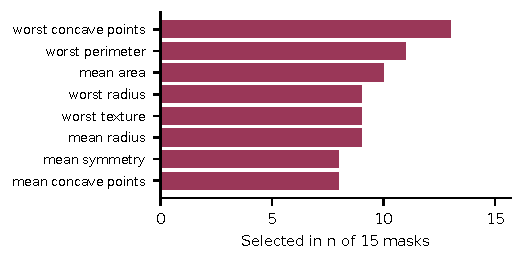
\includegraphics[width=\linewidth]{figures/breast_top_frequencies.pdf}\par{\footnotesize Figure 2. Top eight feature selection counts in fifteen resampled-repair masks.\par}\end{minipage}\par
The shared-service scenario uses published Montana FNA interpretation code 88173: global USD 164.34, effective June 30, 2024 [17]. All 30 WDBC columns derive from FNA images [15]; mapping them to one acquisition group is an illustrative assumption, not a validated invoice. All 75 nonempty primary breast-cancer masks retain the full shared fee: zero service-fee savings and no feasible nonempty subset at a 30\% group budget. Collection, computation time, risk and marginal charges are unknown.

Transfer protocol 7f716c5 preceded 25 source-only fits. Oxford195 training uses grouped inner splits; target UCI489 has 240 recordings/80 subjects (40 PD/40 control) [16]. Only RPDE/DFA/PPE are shared; equal synthetic costs allow repairs one feature. Five-seed probabilities and then three recordings per subject are averaged at threshold 0.5. Target labels serve evaluation only. The 10000-resample stratified subject intervals are descriptive and conditional on fitted models, excluding training uncertainty.

\par\vspace{3pt}\begin{minipage}{\linewidth}{\footnotesize Table 9. External three-feature transfer; five-seed subject ensembles. E=EHOA; R/C/M/S are repairs. BA intervals include 0.5; no clinical superiority.\par}
{\fontsize{6.8}{8.3}\selectfont\setlength{\tabcolsep}{2pt}\renewcommand{\arraystretch}{1.1}
\begin{tabularx}{\linewidth}{>{\hsize=1.0000\hsize\raggedright\arraybackslash}X>{\hsize=1.0000\hsize\raggedright\arraybackslash}X>{\hsize=1.0000\hsize\raggedright\arraybackslash}X>{\hsize=1.0000\hsize\raggedright\arraybackslash}X}\toprule
Methods & BA [95\% descriptive] & Sens./Spec. & AUC\\\midrule
E & 0.575 [0.475,0.675] & 0.725/0.425 & 0.5794\\
R/C/M/S & 0.575 [0.475,0.675] & 0.725/0.425 & 0.5500\\
\bottomrule\end{tabularx}}
\end{minipage}\par\vspace{3pt}
\sect{9  Limitations and reproducibility}
Finite search cannot prove convergence; factorial and larger-search contrasts use one seed. Marginal MI minus SD has no calibrated coverage or false-selection guarantee. Timings use three/six workers. Original recording identity and missing historical records remain unverified. The three-feature transfer uses matching names, without certified extraction/calibration equivalence; it cannot validate the original 22-feature model or prospective clinical use.

github.com/Amirgh23/coststable-ehoa provides code, data and audits. All 1464 final classifiers and 25 transfer predictions were refitted without prediction disagreements; 75 selected optimizer replays matched historical masks. These are current-runtime checks, not recovered historical logs or an exhaustive search replay.

\sect{10  Conclusion}
Fold-local repair enforces synthetic budgets. No-search filters have substantially higher descriptive subset stability; EHOA predictive superiority and necessity are unestablished. Findings are conditional on one synthetic cost vector per dimension and this KNN/SMOTE protocol. Full clinical validation and measured marginal costs remain absent.

\sect{References}
\begin{minipage}{\linewidth}{\fontsize{7}{8.2}\selectfont [1] R. Jagdhuber, M. Lang, A. Stenzl, J. Neuhaus, and J. Rahnenführer, "Cost-Constrained feature selection in binary classification: adaptations for greedy forward selection and genetic algorithms," BMC Bioinformatics, vol. 21, art. 26, 2020. \url{https://doi.org/10.1186/s12859-020-3361-9}\par}\end{minipage}\par
\begin{minipage}{\linewidth}{\fontsize{7}{8.2}\selectfont [2] S. Nogueira, K. Sechidis, and G. Brown, "On the Stability of Feature Selection Algorithms," Journal of Machine Learning Research, vol. 18, no. 174, pp. 1-54, 2018. \url{https://jmlr.org/papers/v18/17-514.html}\par}\end{minipage}\par
\begin{minipage}{\linewidth}{\fontsize{7}{8.2}\selectfont [3] B. Remeseiro and V. Bolon-Canedo, "A review of feature selection methods in medical applications," Computers in Biology and Medicine, vol. 112, art. 103375, 2019. \url{https://doi.org/10.1016/j.compbiomed.2019.103375}\par}\end{minipage}\par
\begin{minipage}{\linewidth}{\fontsize{7}{8.2}\selectfont [4] A. E. Hegazy, M. A. Makhlouf, O. A. M. Salem, and B. Hafiz, "An enhanced Hiking optimization algorithm for accurate and interpretable feature selection in medical data classification," Cluster Computing, vol. 29, art. 244, 2026. \url{https://doi.org/10.1007/s10586-026-05946-9}\par}\end{minipage}\par
\begin{minipage}{\linewidth}{\fontsize{7}{8.2}\selectfont [5] V. Hamer and P. Dupont, "An Importance Weighted Feature Selection Stability Measure," Journal of Machine Learning Research, vol. 22, no. 116, pp. 1-57, 2021. \url{https://jmlr.org/papers/v22/20-366.html}\par}\end{minipage}\par
\begin{minipage}{\linewidth}{\fontsize{7}{8.2}\selectfont [6] T. Klonecki and P. Teisseyre, "Feature selection under budget constraint in medical applications: analysis of penalized empirical risk minimization methods," Applied Intelligence, vol. 53, pp. 29943-29973, 2023. \url{https://doi.org/10.1007/s10489-023-05063-9}\par}\end{minipage}\par
\begin{minipage}{\linewidth}{\fontsize{7}{8.2}\selectfont [7] M. Valancius, M. Lennon, and J. Oliva, "Acquisition Conditioned Oracle for Nongreedy Active Feature Acquisition," Proceedings of the 41st International Conference on Machine Learning, PMLR, vol. 235, pp. 48957-48975, 2024. \url{https://proceedings.mlr.press/v235/valancius24a.html}\par}\end{minipage}\par
\begin{minipage}{\linewidth}{\fontsize{7}{8.2}\selectfont [8] T. Klonecki, P. Teisseyre, and J. Lee, "Cost-Constrained Multi-label Group Feature Selection Using Shadow Features," in Advances in Artificial Intelligence Research, PP-RAI 2025, Lecture Notes in Networks and Systems, vol. 1599, pp. 3-16, Springer, 2026. \url{https://doi.org/10.1007/978-3-032-04197-5_1}\par}\end{minipage}\par
\begin{minipage}{\linewidth}{\fontsize{7}{8.2}\selectfont [9] N. Meinshausen and P. Buhlmann, "Stability selection," Journal of the Royal Statistical Society: Series B, vol. 72, no. 4, pp. 417-473, 2010. \url{https://doi.org/10.1111/j.1467-9868.2010.00740.x}\par}\end{minipage}\par
\begin{minipage}{\linewidth}{\fontsize{7}{8.2}\selectfont [10] R. D. Shah and R. J. Samworth, "Variable selection with error control: another look at stability selection," Journal of the Royal Statistical Society: Series B, vol. 75, no. 1, pp. 55-80, 2013. \url{https://doi.org/10.1111/j.1467-9868.2011.01034.x}\par}\end{minipage}\par
\begin{minipage}{\linewidth}{\fontsize{7}{8.2}\selectfont [11] B. C. Ross, "Mutual Information between Discrete and Continuous Data Sets," PLOS ONE, vol. 9, no. 2, art. e87357, 2014. \url{https://doi.org/10.1371/journal.pone.0087357}\par}\end{minipage}\par
\begin{minipage}{\linewidth}{\fontsize{7}{8.2}\selectfont [12] N. V. Chawla, K. W. Bowyer, L. O. Hall, and W. P. Kegelmeyer, "SMOTE: Synthetic Minority Over-sampling Technique," Journal of Artificial Intelligence Research, vol. 16, pp. 321-357, 2002. \url{https://doi.org/10.1613/jair.953}\par}\end{minipage}\par
\begin{minipage}{\linewidth}{\fontsize{7}{8.2}\selectfont [13] S. Varma and R. Simon, "Bias in error estimation when using cross-validation for model selection," BMC Bioinformatics, vol. 7, art. 91, 2006. \url{https://doi.org/10.1186/1471-2105-7-91}\par}\end{minipage}\par
\begin{minipage}{\linewidth}{\fontsize{7}{8.2}\selectfont [14] J. Demšar, "Statistical Comparisons of Classifiers over Multiple Data Sets," Journal of Machine Learning Research, vol. 7, pp. 1-30, 2006. \url{https://jmlr.org/papers/v7/demsar06a.html}\par}\end{minipage}\par
\begin{minipage}{\linewidth}{\fontsize{7}{8.2}\selectfont [15] W. Wolberg, O. Mangasarian, N. Street, and W. Street, "Breast Cancer Wisconsin (Diagnostic)," UCI Machine Learning Repository, 1993. \url{https://doi.org/10.24432/C5DW2B}\par}\end{minipage}\par
\begin{minipage}{\linewidth}{\fontsize{7}{8.2}\selectfont [16] C. Prez, "Parkinson Dataset with replicated acoustic features," UCI, 2016. \url{https://doi.org/10.24432/C5701F}\par}\end{minipage}\par
\begin{minipage}{\linewidth}{\fontsize{7}{8.2}\selectfont [17] Montana DPHHS, "Cancer Control Programs Fee for Service Schedule," effective June 30, 2024,p.3,code 88173. \url{https://dphhs.mt.gov/assets/publichealth/Cancer/MCCP2025FeeSchedule.pdf}\par}\end{minipage}\par
\begin{minipage}{\linewidth}{\fontsize{7}{8.2}\selectfont [18] R. Jagdhuber and J. Rahnenführer, "Implications on Feature Detection when using the Benefit-Cost Ratio," arXiv:2008.05163v2, 2020. \url{https://doi.org/10.48550/arXiv.2008.05163}\par}\end{minipage}\par
\end{multicols}
\end{document}